\documentclass[10pt]{exam}

\usepackage[margin=1in]{geometry}
\usepackage{amsmath}
\usepackage{amssymb}
\usepackage{amsthm}
\usepackage{mathtools}
\usepackage{bm}
\usepackage{stmaryrd}
\usepackage{booktabs}

\usepackage{color}
\usepackage{colortbl}
\definecolor{deepblue}{rgb}{0,0,0.5}
\definecolor{deepred}{rgb}{0.6,0,0}
\definecolor{deepgreen}{rgb}{0,0.5,0}
\definecolor{gray}{rgb}{0.7,0.7,0.7}

\usepackage{hyperref}
\hypersetup{
  colorlinks   = true, %Colours links instead of ugly boxes
  urlcolor     = black, %Colour for external hyperlinks
  linkcolor    = blue, %Colour of internal links
  citecolor    = blue  %Colour of citations
}

\usepackage{listings}
\lstset{
    basicstyle={\ttfamily}
}

%%%%%%%%%%%%%%%%%%%%%%%%%%%%%%%%%%%%%%%%%%%%%%%%%%%%%%%%%%%%%%%%%%%%%%%%%%%%%%%%

\theoremstyle{definition}
\newtheorem{problem}{Problem}
\newtheorem{example}{Example}
\newtheorem{lemma}{Lemma}
\newtheorem{corollary}{Corollary}
\newtheorem{note}{Note}
\newtheorem{defn}{Definition}
\newtheorem{fact}{Fact}
\newtheorem{refr}{References}
\newtheorem{theorem}{Theorem}
\newcommand{\E}{\mathbb E}
\newcommand{\R}{\mathbb R}
\DeclareMathOperator{\nnz}{nnz}
\DeclareMathOperator{\sign}{sign}
\DeclareMathOperator{\determinant}{det}
\DeclareMathOperator{\Var}{Var}
\DeclareMathOperator{\rank}{rank}
\DeclareMathOperator{\prob}{\mathbb P}
\DeclareMathOperator*{\argmin}{arg\,min}
\DeclareMathOperator*{\argmax}{arg\,max}

\newcommand{\Ein}{E_{\text{in}}}
\newcommand{\Eout}{E_{\text{out}}}
\newcommand{\Etest}{E_{\text{test}}}
\newcommand{\I}{\mathbf I}
\newcommand{\Q}{\mathbf Q}
\newcommand{\p}{\mathbf P}
\newcommand{\pb}{\bar {\p}}
\newcommand{\pbb}{\bar {\pb}}
\newcommand{\pr}{\bm \pi}

\newcommand{\trans}[1]{{#1}^{T}}
\newcommand{\loss}{\ell}
\newcommand{\w}{\mathbf w}
\newcommand{\wstar}{{\w}^{*}}
\newcommand{\x}{\mathbf x}
\newcommand{\y}{\mathbf y}
\newcommand{\lone}[1]{{\lVert {#1} \rVert}_1}
\newcommand{\ltwo}[1]{{\lVert {#1} \rVert}_2}
\newcommand{\lp}[1]{{\lVert {#1} \rVert}_p}
\newcommand{\linf}[1]{{\lVert {#1} \rVert}_\infty}
\newcommand{\lF}[1]{{\lVert {#1} \rVert}_F}

\newcommand{\mH}{m_{\mathcal H}}
\newcommand{\dvc}{{d_{\text{VC}}}}
\newcommand{\HH}[1]{\mathcal H_{\text{#1}}}
\newcommand{\Hbinary}{\HH_{\text{binary}}}
\newcommand{\Haxis}{\HH_{\text{axis}}}
\newcommand{\Hperceptron}{\HH_{\text{perceptron}}}


\newcommand{\ignore}[1]{}

%%%%%%%%%%%%%%%%%%%%%%%%%%%%%%%%%%%%%%%%%%%%%%%%%%%%%%%%%%%%%%%%%%%%%%%%%%%%%%%%

\begin{document}


\begin{center}
{
\Huge
Transfer Learning on Image Data
}
\end{center}

The purpose of this set of notes is to give you background information for your next programming assignment.

\section{Assignment}

Create a program that classifies images of bees versus ants.
You should follow the PyTorch tutorial on ``Transfer Learning for Computer Vision'' located at

\url{https://pytorch.org/tutorials/beginner/transfer_learning_tutorial.html}

\noindent
I strongly recommend working through the ``Introduction to PyTorch'' tutorials before completing this tutorial.
Start with the ``Tensors'' tutorial and work your way through the ``Save and Load a Model'' tutorial.

At the end of the transfer learning tutorial, you will generate a figure demonstrating the output of your code.
You should upload your completed python file and this image to sakai.

The due date is next Sunday (20 Nov).

\section{Image Data}

Bees vs Ants:

\begin{itemize}
\item 2 classes

\item 398 images

\item Pre-determined train/validation split (245/153 images)
\end{itemize}

\noindent
ImageNet dataset:

\begin{itemize}
    \item 1000 classes, 1.2 million images

    \item test set size = 150,000

\end{itemize}

\noindent
Image data is usually ``noisy''

\begin{itemize}
    \item Non-statistical ``noise''

        \begin{itemize}
            \item images are all of different resolutions

            \item size of the bug is different for each image

            \item some images have effects applied to them
        \end{itemize}

    \item Statistical ``noise''

        \begin{itemize}
            \item scraped from the web, so there's errors
            \item human annotations, and humans make mistakes

                Karpathy: human error rate is about 5\%

                \hspace{-0.5in}\url{http://karpathy.github.io/2014/09/02/what-i-learned-from-competing-against-a-convnet-on-imagenet/}

            \item some images can legitimately have multiple labels

                Reference: \url{https://www.unite.ai/assessing-the-historical-accuracy-of-imagenet/}
        \end{itemize}
\end{itemize}


\newpage
\section{Deep Learning}

Reference: \url{https://cs231n.github.io/}

\begin{itemize}
    \item All famous deep learning image classification models are all trained on ImageNet

    \item ImageNet performance change over time:

        \url{https://paperswithcode.com/sota/image-classification-on-imagenet}

    \item Best results use ensembles of deep learning algorithms

        For example: ``Deep Residual Learning for Image Recognition''
\end{itemize}

\noindent
What deep learning looks like:

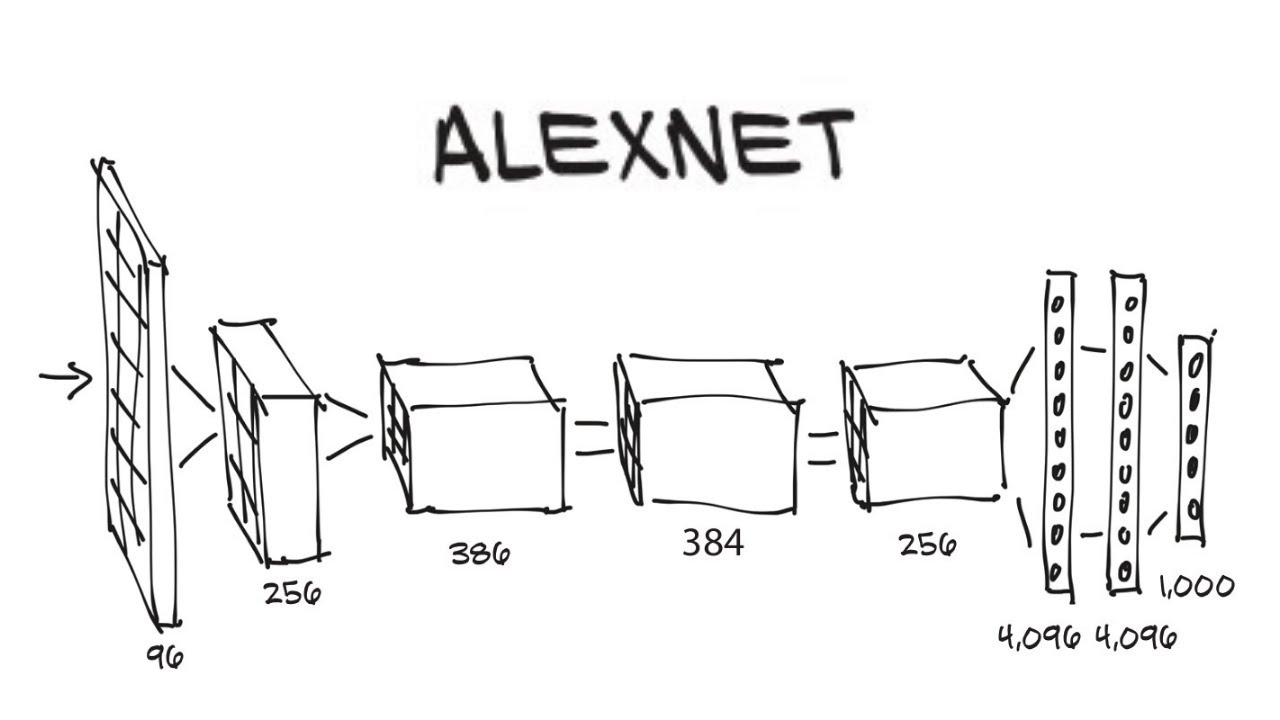
\includegraphics[height=2in]{alexnet}

\vspace{4in}
See also ResNet: ``Deep Residual Learning for Image Recognition''

\newpage
\noindent
Theoretical Problems
\begin{itemize}
    \item Optimization: Highly non-convex optimization problems
        \vspace{1in}

    \item Statistical: VERY high VC dimensions

    VC dimensions are VERY difficult to directly compute,
    so people typically report the number of parameters used in the model as a ``proxy'' for the VC dimension.

        \vspace{2in}

    %Models implemented in pytorch: \url{https://pytorch.org/vision/stable/models.html}

    Double Descent
        Reference: \url{https://medium.com/mlearning-ai/double-descent-8f92dfdc442f}

        \vspace{1.5in}
        \hspace{4in}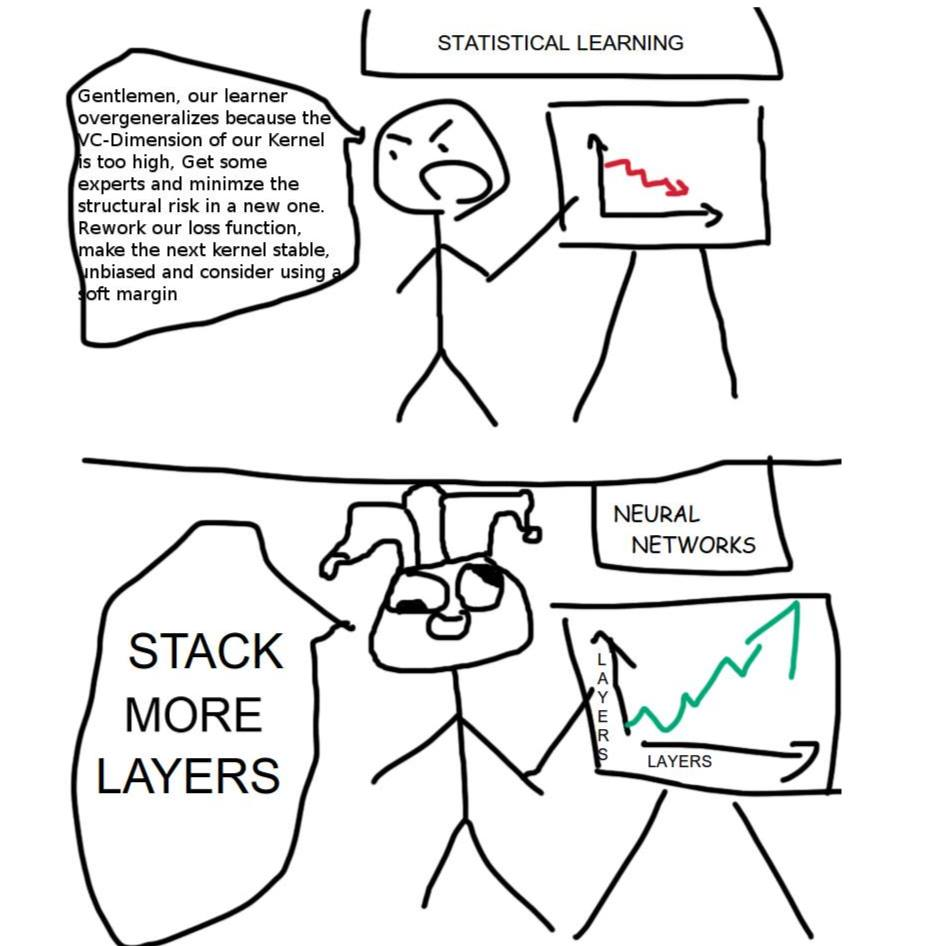
\includegraphics[height=3in]{stack_layers}
        \vspace{-1in}
\end{itemize}

\newpage
\section{Tricks for our dataset}

Three tricks:
\begin{enumerate}
    \item Use an ImageNet-trained CNN for feature extraction

        \begin{itemize}
            \item ``transfer knowledge'' from the ImageNet task to the bees vs ants task
                \vspace{1in}

            \item greatly reduces the VC dimension

                \vspace{3in}

  %VC theory predicts that all networks with the same output dimension will have the same generalization error;
  %networks with better $\Eout$ on ImageNet will tend to have better $\Ein$ on your image classification task

  %The example documentation uses ResNet18,
  %but you'll get better accuracy if you ``upgrade'' to ResNet152 since this has better $\Ein$ with the same generalization error.
  %The downside is that the runtime will be much longer.

            \item Computational notes:
                
                %this is just logistic regression, so the problem is convex, and no need to worry about optimization error/tuning the optimization algorithm

                \begin{itemize}
                    \item pytorch's \lstinline{CrossEntropyLoss} is the logistic loss
                    \item Lots of variations of SGD (Momentum, Adam, AdaGrad)
                    \item Batch size
                    \item Learning rate scheduler
                    \item Still expensive computationally
                \end{itemize}
        \end{itemize}

        \newpage
\item
Solution 2: dataset augmentation

        \begin{itemize}
            \item Reference: \url{http://d2l.ai/chapter_computer-vision/image-augmentation.html}

            \item ``effective number of data points'' equals number of epochs times training set size

            \item technically these new data points are not independent,
  and so we're not ``really'' increasing our dataset in the VC dimension sense... but it's really close and works well in practice

        \end{itemize}

  \item
Solution 3: add regularization
        \begin{itemize}
            \item weight decay
            \item early stopping
            \item dropout
            \item residual layers
            \item batch normalization
        \end{itemize}

\end{enumerate}

%\section{Problems}
%
%\begin{problem}
    %You are working on an image classification problem.
%\end{problem}

\end{document}



